% Declare the wide figure early so it can appear at the top of page two.
\begin{figure*}[t]
    \centering
    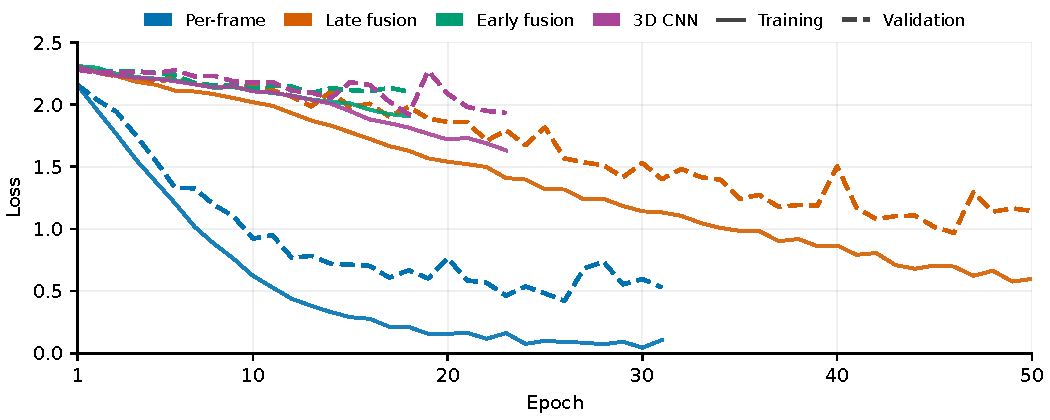
\includegraphics[width=\textwidth]{figures/train_val_loss.pdf}
    \caption{Training (solid) and validation (dashed) loss for all four
    cluster runs on one set of axes ($224\times224$, seed 42, original
    splits). Colour identifies the model. Curves show unsmoothed epoch
    means and end when training stops. Per-frame training uses frame
    cross-entropy (CE); validation uses video negative log-likelihood after
    probability averaging. The other models use video CE for both splits.
    Epochs represent different numbers of optimizer updates.}
    \label{fig:learning}
\end{figure*}

\section{Method}
\label{sec:method}

\paragraph{Shared 2D backbone.}
The per-frame encoder contains three $3\times3$ convolutions with
32, 64, and 128 output channels. Each convolution uses stride one and
padding one, followed by ReLU and $2\times2$ max pooling. Global spatial
average pooling produces a 128-dimensional feature vector, and a linear
layer maps it to ten class logits. The baseline models use no normalization
layers. Let $h(x_t)$ denote the feature vector of frame $t$, and let
$z_t=Wh(x_t)+b$ denote its logits.

\paragraph{Per-frame aggregation.}
Each frame is trained with its video's action label using cross-entropy.
At inference, the video prediction averages the ten frame probability
vectors:
\begin{equation}
    p_{\mathrm{frame}}(y\mid V)
    = \frac{1}{T}\sum_{t=1}^{T}\operatorname{softmax}(z_t)_y,
    \qquad T=10.
\end{equation}
The predicted class is the maximum-probability class. Validation loss is
the negative log-likelihood of this averaged distribution. The model ignores
frame order.

\paragraph{Late fusion.}
The same encoder processes all frames with shared weights. Their features
are averaged before the linear classifier:
\begin{equation}
    p_{\mathrm{late}}(y\mid V)
    = \operatorname{softmax}\!\left(
        W\frac{1}{T}\sum_{t=1}^{T}h(x_t)+b\right)_y.
\end{equation}
Training uses cross-entropy on one logit vector per video. With this linear
classifier, averaging features is equivalent to averaging logits, but is
generally different from averaging probabilities. Mean fusion also ignores
frame order. Its parameter count equals that of the per-frame model.

\paragraph{Early fusion.}
The ten RGB frames are stacked into a 30-channel image in temporal order.
The first convolution is widened to accept these channels; the rest of the
2D backbone is unchanged. This allows frames to interact from the first
layer and makes their ordering relevant. Time is represented by channels,
so the network requires a fixed number of frames and does not slide a
convolutional kernel along time.

\paragraph{3D CNN.}
The clip retains its $3\times T\times H\times W$ representation. Three
$3\times3\times3$ convolutions with padding one produce 32, 64, and 128
channels. Each is followed by ReLU and $1\times2\times2$ max pooling,
preserving temporal resolution while reducing spatial resolution. Global
spatiotemporal average pooling and a linear classifier produce video logits.
The temporal kernels learn local interactions between the sampled frames.
Both early fusion and the 3D CNN use video-level cross-entropy.
